% !TeX root = ../../script.tex
\documentclass[../../script.tex]{subfiles}

\begin{document}
\section{Product measures and Fubini's Theorem}

\begin{eg}
    Let 
    \[
        f: [0, 1] \times [0, 1] \longrightarrow [0, \infty)
    \]
    Question: What is the volume (or the $\lambda^2$ measure) under the graph of $f$, i.e.
    \[
        \set[0 \le z \le f(x, y)]{(x, y, z) \in \realn^3}
    \]
    The possibilities are 
    \begin{gather*}
        \int f \dd\lambda^2 \\
        \int_0^1 \int_0^1 f(x, y) \dd x \dd y ~~\text{ or }~~ \int_0^1 \int_0^1 f(x, y) \dd y \dd x
    \end{gather*}
\end{eg}
From now on we define $\measure$ and $(\Phi, \setfamb, \nu)$ to be measure spaces.
\begin{defi}
    The product $\sigma$-algebra $\setfam \otimes \setfamb$ is the smallest $\sigma$-algebra on $\Omega \times \Phi$ that contains
    all sets of type $A \times B$ for $A \in \setfam, B \in \setfamb$.

    Examples for $A \times B$ are 

    \begin{center}
        \begin{minipage}{.49\linewidth}
            \begin{center}
                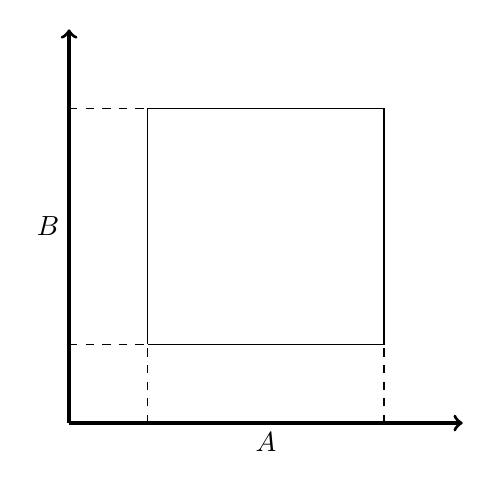
\begin{tikzpicture}
                    \draw[very thick, ->] (0, 0) -- (5, 0);
                    \draw[very thick, ->] (0, 0) -- (0, 5);

                    \draw (1, 1) -- (4, 1) -- (4, 4) -- (1, 4) -- (1, 1);

                    \draw[dashed] (0, 4) -- (1, 4);
                    \draw[dashed] (0, 1) -- (1, 1);
                    \draw[dashed] (1, 0) -- (1, 1);
                    \draw[dashed] (4, 0) -- (4, 1);

                    \node[below] at (2.5, 0) {$A$};
                    \node[left] at (0, 2.5) {$B$};
                \end{tikzpicture}
            \end{center}
        \end{minipage}
        \begin{minipage}{.49\linewidth}
            \begin{center}
                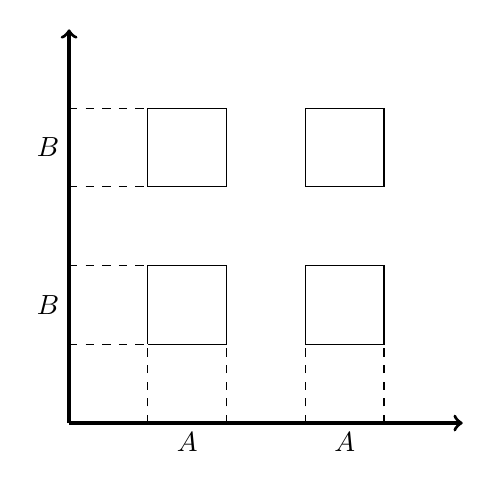
\begin{tikzpicture}
                    \draw[very thick, ->] (0, 0) -- (5, 0);
                    \draw[very thick, ->] (0, 0) -- (0, 5);

                    \draw (1, 1) -- (2, 1) -- (2, 2) -- (1, 2) -- (1, 1);
                    \draw (3, 1) -- (4, 1) -- (4, 2) -- (3, 2) -- (3, 1);
                    \draw (1, 3) -- (2, 3) -- (2, 4) -- (1, 4) -- (1, 3);
                    \draw (3, 3) -- (4, 3) -- (4, 4) -- (3, 4) -- (3, 3);

                    \draw[dashed] (0, 4) -- (1, 4);
                    \draw[dashed] (0, 3) -- (1, 3);
                    \draw[dashed] (0, 2) -- (1, 2);
                    \draw[dashed] (0, 1) -- (1, 1);
                    \draw[dashed] (4, 0) -- (4, 1);
                    \draw[dashed] (3, 0) -- (3, 1);
                    \draw[dashed] (2, 0) -- (2, 1);
                    \draw[dashed] (1, 0) -- (1, 1);

                    \node[left] at (0, 3.5) {$B$};
                    \node[left] at (0, 1.5) {$B$};
                    \node[below] at (1.5, 0) {$A$};
                    \node[below] at (3.5, 0) {$A$};
                \end{tikzpicture}
            \end{center}
        \end{minipage}
    \end{center}
    \pagebreak NO examples for $A \times B$ are 

    \begin{center}
        \begin{minipage}{.49\linewidth}
            \begin{center}
                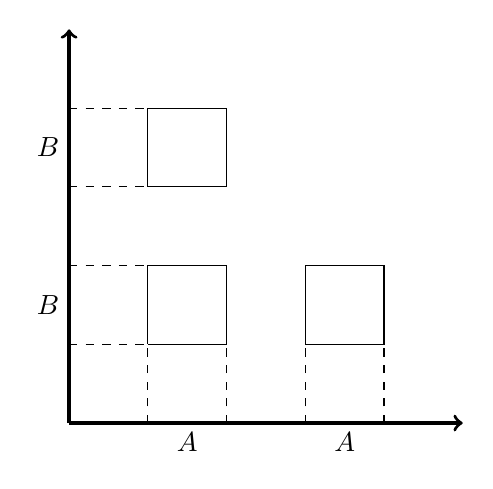
\begin{tikzpicture}
                    \draw[very thick, ->] (0, 0) -- (5, 0);
                    \draw[very thick, ->] (0, 0) -- (0, 5);

                    \draw (1, 1) -- (2, 1) -- (2, 2) -- (1, 2) -- (1, 1);
                    \draw (3, 1) -- (4, 1) -- (4, 2) -- (3, 2) -- (3, 1);
                    \draw (1, 3) -- (2, 3) -- (2, 4) -- (1, 4) -- (1, 3);

                    \draw[dashed] (0, 4) -- (1, 4);
                    \draw[dashed] (0, 3) -- (1, 3);
                    \draw[dashed] (0, 2) -- (1, 2);
                    \draw[dashed] (0, 1) -- (1, 1);
                    \draw[dashed] (4, 0) -- (4, 1);
                    \draw[dashed] (3, 0) -- (3, 1);
                    \draw[dashed] (2, 0) -- (2, 1);
                    \draw[dashed] (1, 0) -- (1, 1);

                    \node[left] at (0, 3.5) {$B$};
                    \node[left] at (0, 1.5) {$B$};
                    \node[below] at (1.5, 0) {$A$};
                    \node[below] at (3.5, 0) {$A$};
                \end{tikzpicture}
            \end{center}
        \end{minipage}
        \begin{minipage}{.49\linewidth}
            \begin{center}
                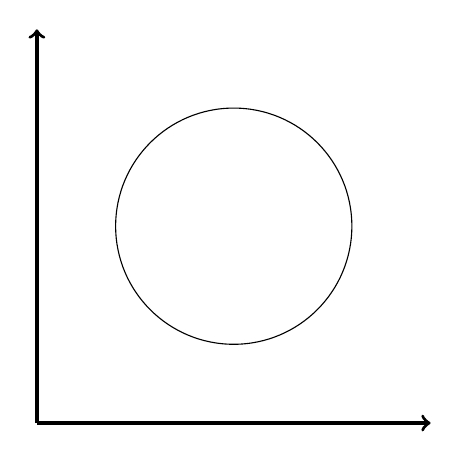
\begin{tikzpicture}
                    \draw[very thick, ->] (0, 0) -- (5, 0);
                    \draw[very thick, ->] (0, 0) -- (0, 5);

                    \draw (2.5, 2.5) circle[radius=1.5];

                    \node[below] at (0, 0) {\quad};
                \end{tikzpicture}
            \end{center}
        \end{minipage}
    \end{center}
    A measure $\vartheta$ defined on $\setfam \otimes \setfamb$ is said to be a product measure of $\mu, \nu$ if 
    \[
        \vartheta(A \times B) = \mu(A) \nu(B) ~~A \in \setfam, B \in \setfamb
    \]
\end{defi}

\begin{rem}
    Product measures always exist. For $\sigma$-finite measure spaces they are unique. Notation:
    \[
        \mu \otimes \nu ~~\text{ or }~~ \mu^2 = \mu \otimes \mu
    \]
\end{rem}

\begin{eg}
    $\realn$ with Lebesgue measure $\lambda$. $\lambda^2$ is the product measure on $\realn^2$.
    \begin{align*}
        \lambda^2([a, b] \times [c, d]) &= \lambda([a, b])\lambda([c, d]) \\
        &= (b - a)(d - c)
    \end{align*}
    This means the product measure characterizes the area. Analogously this can be extended for $\lambda^3$, $\lambda^4$ etc.
\end{eg}

\begin{eg}
    Consider 
    \begin{align*}
        f: \realn^2 &\longrightarrow \realn \\
        f &= \sum_{n=0}^{\infty} \left(\charfun_{[n, n+1)^2} - \charfun_{[n+1, n+2) \times [n, n+1)}\right)
    \end{align*}

    \begin{center}
        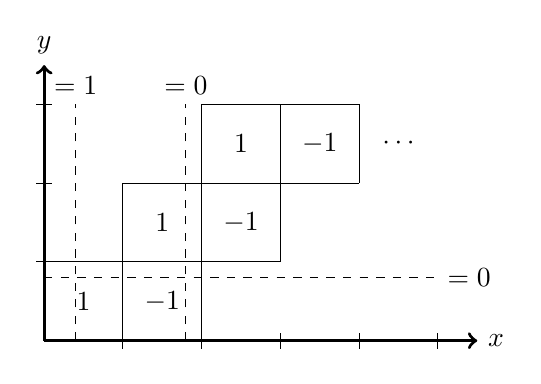
\begin{tikzpicture}
            \draw[->, very thick] (0, 0) -- (0, 3.5) node[above] {$y$};
            \draw[->, very thick] (0, 0) -- (5.5, 0) node[right] {$x$};

            \foreach \x in {1,...,5} \draw (\x, -0.1) -- (\x, 0.1);
            \foreach \y in {1,...,3} \draw (-0.1, \y) -- (0.1, \y);

            \draw (0, 1) -- (3, 1);
            \draw (1, 2) -- (4, 2);
            \draw (2, 3) -- (4, 3);
            \draw (1, 2) -- (1, 0);
            \draw (2, 3) -- (2, 0);
            \draw (3, 3) -- (3, 1);
            \draw (4, 3) -- (4, 2);

            \node at (4.5, 2.5) {$\cdots$};
            \node at (0.5, 0.5) {$1$};
            \node at (1.5, 0.5) {$-1$};
            \node at (1.5, 1.5) {$1$};
            \node at (2.5, 1.5) {$-1$};
            \node at (2.5, 2.5) {$1$};
            \node at (3.5, 2.5) {$-1$};

            \draw[dashed] (0, 0.8) -- (5, 0.8) node[right] {$=0$};
            \draw[dashed] (0.4, 0) -- (0.4, 3) node[above] {$=1$};
            \draw[dashed] (1.8, 0) -- (1.8, 3) node[above] {$=0$};
        \end{tikzpicture}
    \end{center}
    \begin{align*}
        \iint f(x, y) \dd x \dd y = 0 && \iint f(x, y) \dd y \dd x = 1
    \end{align*}
    But the integral $\int f \dd\lambda^2$ doesn't exist
    \[
        \int \abs{f} \dd\lambda^2 = \sum_{n=0}^{\infty} 2 = \infty 
    \]
\end{eg}

\begin{thm}[Tonelli's Theorem]
    Let $f: \Omega \times \Phi \rightarrow [0, \infty)$ be measurable (in terms of $\setfam \otimes \setfamb$).
    Then the functions
    \[
        \omega \longmapsto f(\omega, \phi)
    \]
    are measurable for almost all $\phi \in \Phi$. Analogously
    \[
        \phi \longmapsto f(\omega, \phi)
    \]
    is measurable for almost all $\omega \in \Omega$.
    \begin{align*}
        \phi &\longmapsto \int f(\omega, \phi) \dd\mu(\omega) \text{ measurable} \\
        \omega &\longmapsto \int f(\omega, \phi) \dd\mu(\phi) \text{ measurable}
    \end{align*}
    and 
    \begin{align*}
        \int f(\omega, \phi) \dd (\mu \otimes \nu) (\omega, \phi) &= \iint f(\omega, \phi) \dd\mu(\omega) \dd\nu(\phi) \\
        &= \iint f(\omega, \phi) \dd\nu(\phi) \dd\mu(\omega)
    \end{align*}
    Furthermore, $f$ is integrable in terms of $\mu \otimes \nu$ is one of the above integrals is finite.
\end{thm}
\begin{proof}
    Without proof.
\end{proof}

\begin{cor}[Cavalieri's Principle]
    Let $A \subset \setfam \otimes \setfamb$. Define 
    \[
        A_{\omega} = \set[(\omega, \phi) \in A]{\phi \in \Phi}
    \]
    Then 
    \[
        \omega \longmapsto \nu(A_{\omega})
    \]
    is measurable and 
    \[
        (\mu \otimes \nu)(A) = \int \nu(A_{\omega}) \dd\mu(A_{\omega})
    \]
\end{cor}
\begin{proof}
    It is easy to see
    \begin{equation}
        (\omega, \phi) \in A \iff \phi \in A_{\omega}
    \end{equation}
    Thus we can see 
    \begin{equation}
        \charfun_A(\omega, \phi) = \charfun_{A_{\omega}} (\phi)
    \end{equation}
    And then 
    \begin{equation}
        \begin{split}
            (\mu \otimes \nu)(A) &= \int \charfun_A(\omega, \phi) \dd{(\mu \otimes \nu)}(\omega, \phi) \\
            &= \iint \underbrace{\charfun_A (\omega, \phi)}_{\charfun_{A_{\omega}}(\phi)} \dd{\nu}(\phi) \dd{\mu}(\omega) \\
            &= \int \nu(A_{\omega}) \dd{\mu}(\omega)
        \end{split}
    \end{equation}
\end{proof}

\begin{thm}[Fubini's Theorem]
    Let $f: \Omega \times \Phi \rightarrow \field$ be measurable with measures $\mu, \nu$, which is integrable in terms of $\mu \otimes \nu$.
    Then the functions $\omega \mapsto f(\omega, \phi)$ are measurable and integrable for $\nu$-almost every $\phi \in \Phi$, 
    and the functions $\phi \mapsto f(\omega, \phi)$ are measurable and integrable for $\mu$-almost every $\omega \in \Omega$.
    The functions 
    \begin{align*}
        \omega &\longmapsto \int f(\omega, \phi) \dd{\nu}(\phi) && \phi \longmapsto \int f(\omega, \phi) \dd{\mu}(\omega)
    \end{align*}
    are measurable and integrable, and 
    \begin{align*}
        \int f(\omega, \phi) \dd{(\mu \otimes \nu)} &= \iint f(\omega, \phi) \dd{\nu}(\phi) \dd{\mu}(\omega) \\
        &= \iint f(\omega, \phi) \dd{\mu}(\omega) \dd{\nu}(\phi)
    \end{align*}
\end{thm}
\begin{proof}
    Without proof.
\end{proof}

\begin{cor}
    Let $a_i, b_i \in \realn$, $a_i < b_i ~~\forall i \in \set{1, \cdots, n}$.
    \[
        D = [a_1, b_1] \times [a_2, b_2] \times \cdots \times [a_n, b_n]
    \]
    Let $f: D \rightarrow \realn$ be continuous or bounded. Then 
    \[
        \int_D f \dd{\lambda^n} = \int\limits_{a_1}^{b_1} \cdots \int\limits_{a_n}^{b_n} f(x_1, \cdots, x_n) \dd{x_n} \cdots \dd{x_1}
    \]
    and the order of integration is irrelevant.
\end{cor}
\begin{proof}
    $f$ is bounded by $k \in \realn$ (continuous with compact domain)
    \begin{equation}
        \int_D \abs{f} \dd{\lambda^n} \le \int_D k \dd{\lambda^n} = k \cdot (b_1 - a_1)(b_2 - a_2) \cdots (b_n - a_n) < \infty
    \end{equation}
    $f$ is $\lambda^n$-integrable. By applying Fubini's theorem the desired statement follows.
\end{proof}

\begin{eg}
    Calculate the center of mass of 
    \[
        A = \set[x \ge y^2 \wedge x \le 1]{(x, y) \in \realn^2}
    \]

    \begin{center}
        \begin{tikzpicture}[scale=2]
            \draw[->, thick] (-0.5, 0) -- (3.5, 0);
            \draw[->, thick] (0, -1.2) -- (0, 1.2);

            \draw[domain=-1:1, smooth, variable=\y] plot({3*\y*\y}, {\y});
            \draw[dashed] (3, -1) -- (3, 1);
        \end{tikzpicture}
    \end{center}
    The center of mass is defined by 
    \[
        \int \begin{pmatrix}
            x \\ y
        \end{pmatrix} \underbrace{\dd{\lambda^2}(x, y)}_{\dd A}
    \]
    In component form this is 
    \begin{align*}
        \int_A x \dd{\lambda^2}(x, y) &= \int x \charfun_A(x, y) \dd{\lambda^2}(x, y) \\
        &= \int_{[0, 1] \times [-1, 1]} x \charfun_A(x, y) \dd{\lambda^2}(x, y) \\
        &= \int_0^1 \int_{-1}^1 x \charfun_{[-\sqrt{x}, \sqrt{x}]}(y) \dd{y}\dd{x} \\
        &= \int_0^1 x \cdot 2 \cdot \sqrt{x} \dd{x} = \frac{4}{5}
    \end{align*}
    Meaning the center of mass is at $(\frac{4}{5}, 0)$.
\end{eg}
\end{document}